%% psoc_api

API til styring af PSoC4, herunder sensor og sprinkler, er implementeret i PSoC Creator. Top designet består af en ADC\_SAR\_Seq, en analog pin og to digitale pins til at styre henholdsvis sprinkler og Select til bestemmelse af temperatur- eller fugtighedsdata for SHT21p.
I top designet, se figur \ref{lab:psoc_api_topdesign}, er der angivet følgende pins. ''P\_FT1'', ''P\_FT2'', ''P\_VP'' disse forbindes til henholdsvis pin P2[5], P0[0] og P2[0]. P\_FT1 oprettes som en analog pin og de to andre som digitale output pins. Under konfiguration for de digitale pins fravælges ''HW Connection'' under Digital Output. For nærmere opsætning af pins henvises til figur \ref{lab:P_PV_config} og figur \ref{lab:P_FT2_config}

\begin{figure}[htb]
\centering
{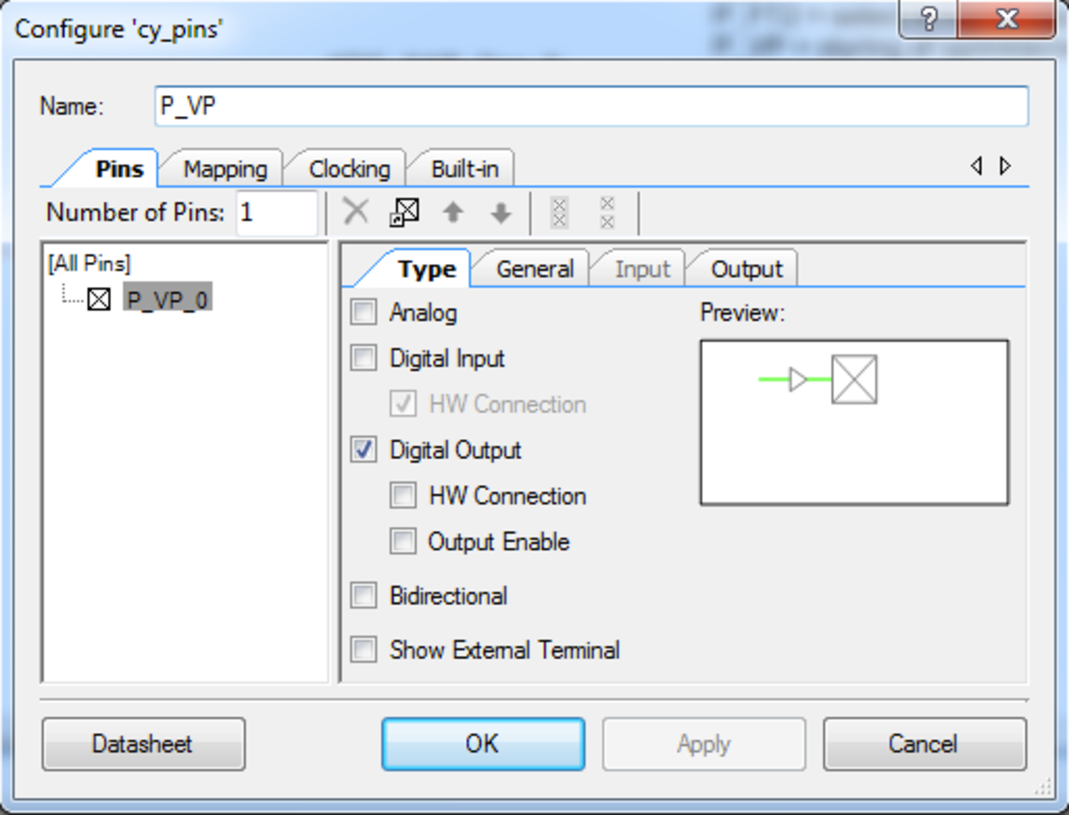
\includegraphics[width=0.70\textwidth]{filer/pics/P_PV_config}}
\caption{Konfiguration for P\_PV}
\label{lab:P_PV_config}
\end{figure}


\begin{figure}[htb]
\centering
{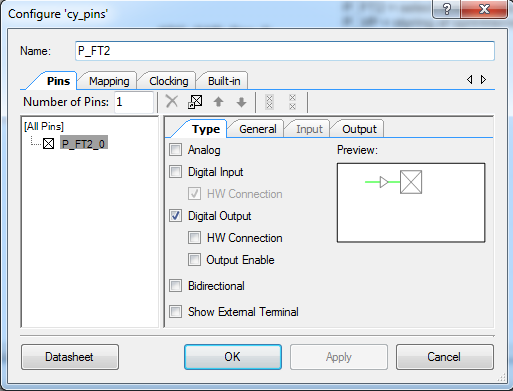
\includegraphics[width=0.70\textwidth]{filer/pics/P_FT2_config}}
\caption{Konfiguration for P\_FT2}
\label{lab:P_FT2_config}
\end{figure}  

Under konfiguration for ADC-komponenten vælges Vref til VDDA og Single ended negative input vælges til Vss. Dette sætter ADCen op til at bruge 0 V som referencespænding.

Da PSoC4 kun har en SAR komponent er det nødvendigt at initialisere denne i sensorPackage-driveren.

\begin{figure}[htb]
\centering
{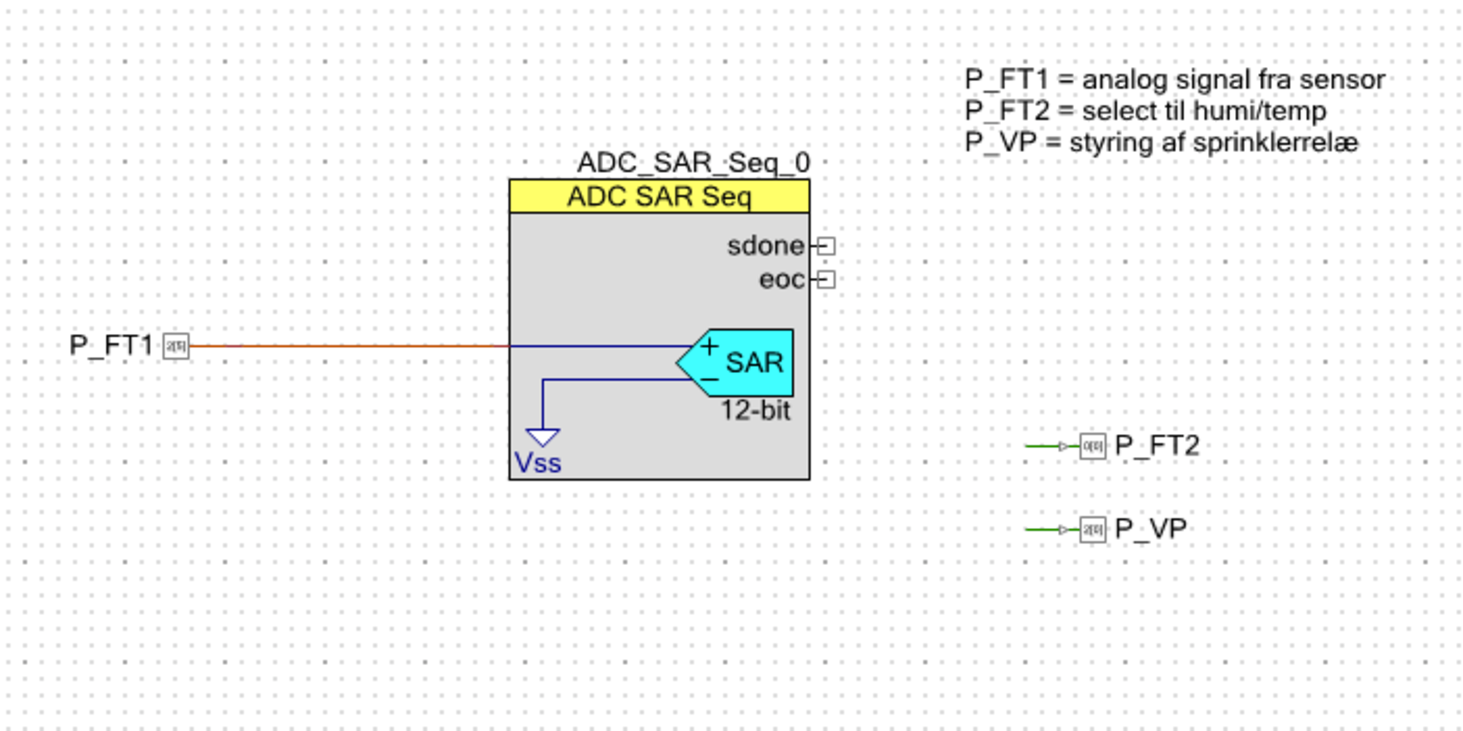
\includegraphics[width=0.70\textwidth]{filer/pics/psoc_api_topdesign}}
\caption{Top Design for PSoC4 API}
\label{lab:psoc_api_topdesign}
\end{figure}

\begin{figure}[htb]
\centering
{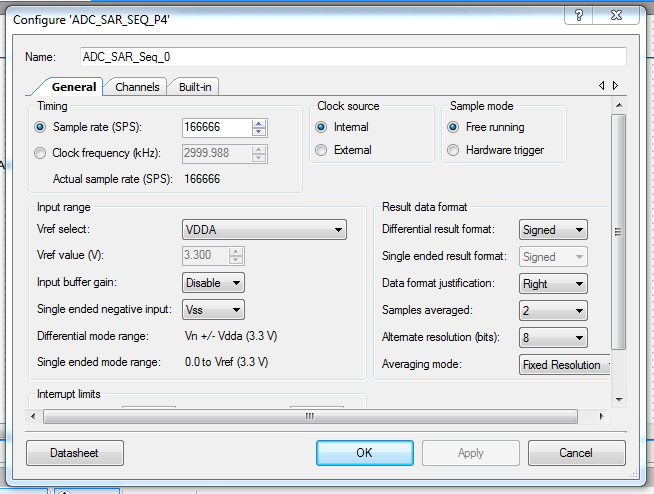
\includegraphics[width=0.70\textwidth]{filer/pics/psoc_api_config1}}
\caption{Konfiguration af Vref og Single ended negative input}
\label{lab:psoc_api_config1}
\end{figure}

\begin{figure}[htb]
\centering
{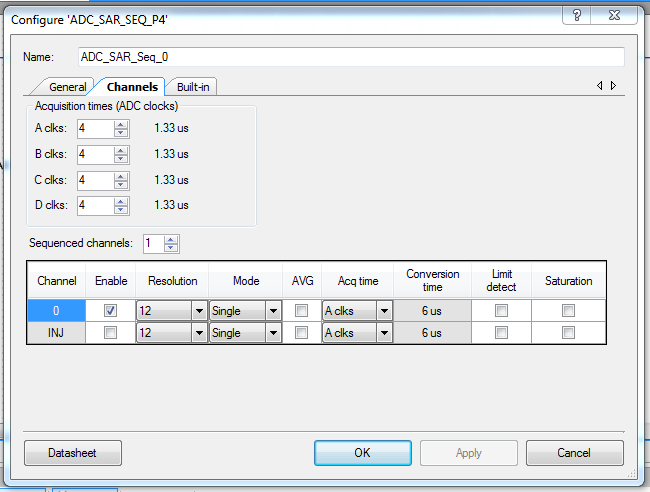
\includegraphics[width=0.70\textwidth]{filer/pics/psoc_api_config2}}
\caption{Konfiguration af Channels for ADC}
\label{lab:psoc_api_config2}
\end{figure}